\documentclass[11pt]{article}
\usepackage[utf8]{inputenc}

% MATH
\usepackage{amssymb}
\usepackage{amsmath}
\usepackage{amsthm}
\usepackage{mathtools}
\usepackage{bm}

\newtheorem{pb}{Problème}
\newtheorem{rmq}{Remarque}

% MISE EN FORME
\usepackage[left=2cm,right=2cm,top=2cm,bottom=2cm]{geometry}

\usepackage{hyperref}
\usepackage{xcolor}
\hypersetup{
	colorlinks,
	linkcolor={red!50!black},
	citecolor={blue!50!black},
	urlcolor={blue!80!black}
}

% MACROS
\usepackage{xparse}
\newcommand{\smbox}[1]{\mbox{\footnotesize #1}}
\newcommand{\Am}{\mathbb{A}}
\newcommand{\N}{\mathbb{N}}
\newcommand{\C}{\mathbb{C}}
\renewcommand{\P}{\mathbb{P}}
\newcommand{\R}{\mathbb{R}}
\newcommand{\M}{\mathbb{M}}
\newcommand{\D}{\mathbb{D}}
\newcommand{\tD}{\widetilde{\mathbb{D}}}
\newcommand{\J}{\mathbb{J}}
\newcommand{\K}{\mathbb{K}}
\newcommand{\Kk}{\mathbb{K}^k}
\newcommand{\Ktk}{\mathbb{K}^{T,k}}
\newcommand{\Ktkc}{\mathbb{K}^{T, k}_c}
\newcommand{\T}{\mathcal{T}}
\newcommand{\Ah}{A^{hom}}
\newcommand{\uh}{u^{hom}}
\newcommand{\bx}{\bar{x}}
\newcommand{\tphi}{\tilde{\phi}}
\newcommand{\Ye}{Y_\varepsilon}
\newcommand{\tw}{\tilde{w}}
\newcommand{\Ae}{A^\varepsilon}
\newcommand{\Be}{B^\varepsilon}
\newcommand{\ue}{u^\varepsilon}
\newcommand{\ie}{\emph{i.e.{}}~}
\newcommand{\st}{\text{~~s.t.~~}}
\newcommand{\norm}[1]{\left|\left|#1\right|\right|}
\newcommand{\sca}[2]{\big<#1, #2\big>}
\newcommand{\cont}[1]{\mathcal{C}^{#1}}
\newcommand{\question}[2]{\paragraph{Question #1.}\textit{#2} \\}
\newcommand{\Hd}{H^1_{\#}}
\newcommand{\td}{\text{d}}
\newcommand{\balpha}{\bm{\alpha}}
\newcommand{\bbeta}{\bm{\beta}}
\newcommand{\blambda}{\bm{\lambda}}
\newcommand{\balphac}{\bm{\alpha}_c}
\newcommand{\bbetac}{\bm{\beta}_c}
\newcommand{\bpsi}{\bm{\psi}}
\newcommand{\xtk}{x_{T,k}}

\newcommand{\funcin}{\item[\textcolor{red}{$\bm{\rightarrow}$}]}
\newcommand{\funcout}{\item[\textcolor{red}{$\bm{\leftarrow}$}]}
\newcommand{\loopin}{\item[\textcolor{blue}{\textbullet}]}
\newcommand{\loopout}{\item[\textcolor{blue}{\textbullet}]}


\title{Rapport TP X01 \\ TP4}
\author{Aurélien Valade}
\date{}

\begin{document}
\maketitle

\section{Introduction}

Dans ce rapport, nous allons nous pencher sur la description et l'implémentation d'un code de résolutions d'équations aux dérivées partielles par méthode
d'éléments finis et résolution hétérogène multi-échelles, termes que nous détaillerons plus loin. Ce travaille se présente en deux parties : tout d'abord
en une analyse du papier de \cite{abdulle2009short}, puis une tentative de ré-implémentation de certaines parties de ce code à l'aide des routines développées
dans les TP précédents. Contrairement au papier qui présente des méthodes pour différents types de maillage en deux ou trois dimensions, nous nous
bornerons à des explications en deux dimensions avec des maillages de simplexes, c'est à dire triangulaires dans notre cas. 

\section{Analyse du papier \& méthodologie du code}

Ce papier a pour but l'implémentation d'un code MATLAB simple et multifonctions à mettre à disposition du publique. Celui ci permettrait la résolution
d'EDP dont la physique amène à considérer des phénomènes physiques couplés sur plusieurs échelles d'espaces distinctes. Pour la résolution de tels
problèmes, une approche frontale serait donc de discrétiser tout l'espace avec un maillage dont les cellules seraient à l'échelle du phénomène physique le
plus petit, mais cela amènerait à d'énormes problèmes numériques très coûteux à résoudre. Parfois la physique demande même à ce que la taille du phénomène
microscopique tende vers zéro, il est alors impossible d'attaquer le problème brutalement et il faut donc créer un meilleur cadre analytique et trouver
des méthodes numériques plus efficaces quitte à faire des approximations.

La littérature semble être fournie en ce qui concerne l'approche analytique de ce genre de problème multi-échelles, cependant peu d'outils numériques
seraient disponibles aujourd'hui, ce à quoi le travail présenté dans ce papier veut remédier en proposant ce code MATLAB court, modulable et parallélisable.

\subsection{Cadre mathématique de la résolution}

\subsubsection{Présentation de l'équation}

L'étude présentée dans ce papier porte sur des méthodes d'éléments finis (FE) pour la résolution de problèmes elliptiques et paraboliques comme suit.

\begin{pb}
  \label{pb:parael}
  Soient les sous espaces $\Omega \subset \R^d$\quad et \quad $Y = [0,1]^d$. Soient $\varepsilon >0$, $\alpha\in \{0, 1\}$ et soient les fonctions sur ces
  espaces $f : \Omega \to \R, \quad \Ae : \Omega\times Y \to \mathcal{M}_d(\R)$  telle que $\Ae  = (\Ae)^T$ \quad et \quad $g_{N,D} : \partial \Omega_{N, D} \to \R$. \\
  Trouver $u$ tel que
  \begin{equation*}
    \begin{cases}
      \alpha \partial_t \ue -\nabla(\Ae \nabla \ue) = f & \text{sur }\Omega\\
      \ue = g_D & \text{sur }\partial \Omega_D \\
      n\cdot(\Ae \nabla \ue) = g_N & \text{sur }\partial \Omega_N
    \end{cases}
  \end{equation*}
\end{pb}

\begin{rmq}
  Il s'agit d'un problème elliptique si $\alpha=0$, sinon il s'agit d'un problème parabolique.
\end{rmq}

\begin{rmq}
  La dépendance en $\varepsilon$ de $\Ae$ n'est pas forcément de la forme vue en cours, \ie périodique $\Ae(x/\varepsilon)$, mais elle peut être
  quasi-périodique $\Ae(x, x/\varepsilon)$, ou bien même implicite, bien qu'on ne considère dans la suite que ce cas simple. Il est cependant nécessaire
  d'avoir pour tout $\varepsilon$ les propriétés suivantes :
  \[
    \exists \lambda, \Lambda > 0 \st \lambda \xi^2 < (\Ae \xi) \cdot \xi < \Lambda \xi^2 \quad \forall \xi \in \R^d
  \]
  en tous points pour pouvoir prouver que le problème variationnel vu en \autoref{sec:pbvar} est bien posé.
\end{rmq}

\begin{rmq}
  Dans notre code on traitera uniquement le cas où $\partial \Omega_N = \emptyset$.
\end{rmq}
Cette formulation permet de mettre en exergue la dépendance en $\varepsilon$ qui est l'échelle la plus petite du problème, et qui tend usuellement
vers zéro. C'est cette dépendance qui est au centre du questionnement. En effet il ne suffit pas de trouver une solution $\ue$ explicite en
$\varepsilon$ et de faire tendre $\varepsilon$ vers zéro pour trouver $u^0$ -- ce qui est de plus impossible analytiquement dans le cas général. La
convergence n'est généralement que faible dans $L^2$ :
\[
  \lim_{\varepsilon \to 0} \int_\Omega \ue \phi = \int_\Omega u^0 \phi \qquad \forall \phi \in L^2(\Omega).
\]

Les deux méthodes présentées plus loin permettent de palier à ce problème par des méthodes analytiques amenant à des implémentations numériques modifiées.


\subsubsection{Problème variationnel associé}
\label{sec:pbvar}

On va poser ici la formulation variationnelle discrète du problème pour mieux voir les éléments qui nous intéressent réellement, à savoir les coefficients
de la matrice de rigidité.

Par une démonstration vue plusieurs fois en cours dans un cadre plus restreint\footnote{Multiplication par $\phi$,
  Green-Ostrogradski deux fois dont la deuxième pour changer l'intégrale sur $g_D$.}, on obtient que le problème \ref{pb:parael} est équivalent à
\begin{equation}
  \underbrace{\int_\Omega (\Ae \nabla \ue)\cdot \nabla \phi}_{\Be(\ue, \phi)} =
  \underbrace{\int_\Omega f \phi + \int_{\partial \Omega_N} g_N \phi - \int_{\Omega} (\Ae \nabla g_D)\cdot \nabla \phi}_{l^{\varepsilon}(\phi)}
  \qquad \forall \phi \in L^2(\Omega).
\end{equation}

\begin{rmq}
  On peut réécrire immédiatement
  \[
    l^{\varepsilon}(\phi) = l(\phi) - \Be(g_D, \phi).
  \]
\end{rmq}

Sous certaines conditions de coercitivité et de continuité des fonctions (bi)linéaires en présence, on peut montrer que le problème est bien posé à l'aide
du théorème de Lax-Milgram.

Il apparaît que le point centrale de la difficulté de cette équation est dans la fonction bilinéaire $\Be$. Ce sont en effet ces coefficients que l'on
cherchera à calculer par la méthode la plus adaptée pour quand $\varepsilon$ tend vers 0.

Avant cela, discrétisons cette équation sur une base finie de fonctions de $L^2(\Omega)$. On se donne un maillage de simplexe en deux
dimensions\footnote{Le papier susmentionné va plus loin en considérant d'autres types de maillages, en 2D et en 3D.}. On note les sommets de ce maillage
les $\{S_i\}_{1, N}$ et $\T_h$ l'ensemble des simplexe. On définit l'ensemble des sommets les fonctions de $\R^g[X]$ avec $g\in\N$ le degré des polynômes
choisi. Ces fonctions, notées $\{\varphi_i\}_{1, N}$ par la suite sont telles que
\[
  \varphi_i(S_j) = \delta_{i,j} \quad \forall i, j \in [1, N]^2.
\]
On projette $\ue$ sur cette bases et on utilise les $\{\varphi_i\}_{1, N}$ comme $\phi$ pour obtenir le système linéaire 
\[
  \K^\varepsilon U^\varepsilon = L^\varepsilon
\]
avec $\K^\varepsilon_{ij} = \Be(\varphi_i, \varphi_j), ~ U^\varepsilon_i = \ue(S_i)$ et $L^\varepsilon_i = l^\varepsilon(\varphi_i)$.


\subsection{Méthode d'homogénéisation classique}
  
Le concept développé en homogénéisation pure est de trouver un méthode pour calculer le tenseur $\Ah$ en tout point pour pouvoir ensuite résoudre le
problème dérivé qui nous donne la solution $\uh=\lim_{\varepsilon\to 0}\ue$:
\begin{pb}
  Trouver $\uh$ tel que
  \begin{equation*}
    \alpha \partial_t \uh -\nabla(\Ah \nabla \uh) = f
  \end{equation*}
\end{pb}


L'avantage est ici que $\varepsilon$ a complètement disparu de l'équation et donc qu'un
maillage adapté aux grandes échelles seules suffit. Cependant il faut pour cela calculer $\Ah(\bx)$ au préalable \ie avant la résolution du macro
problème. Pour cela on résout les problèmes dits de cellule en tout point $\bx \in \Omega$ pour trouver les $\{w_i\}_{1, d}$ : 
\begin{equation}
  \label{eq:cell}
  \int_Y A^1(\bx, y) \nabla w_i(\bx, y) \nabla \phi(y) \td y  = \int_Y A^1(\bx, y) e_i \nabla \phi(y) \td y
  \quad  \forall\phi\in L^2(\Omega) \qquad \forall i \in \{1, d\} 
\end{equation}
puis on calcule le tenseur homogénéisé
\begin{equation}
  \label{eq:Ahom}
  \Ah_{jk}(\bx) = \int_Y A(\bx, y)\big(e_k+\nabla_y w_k(\bx, y)\big)\big(e_j+\nabla_y w_j(\bx, y)\big) \td y 
\end{equation}
et on peut finalement résoudre le système linéaire homogénéisé :
\[
  \K U = L
\]
avec $\K_{ij} = \int_\Omega (\Ah \varphi_i)\cdot \varphi_j, ~ U_i = \uh(S_i)$ et $L_i = l(\varphi_i) - \int_\Omega (\Ah g_D)\cdot \varphi_i$.
\begin{rmq}
  Dans notre cas, $d=2$.
\end{rmq}
Le gros inconvénient de cette méthode étant qui faut préalablement calculer le tenseur homogénéisé $\Ah$ théoriquement en tout point de $\Omega$ de
l'espace discrétisé.


\subsection{Différences et apport de la nouvelle méthode}

La méthode de la FE-HMM (\emph{finite elements heterogenous multi-scale method}) présente tous les avantages d'une méthode d'homogénéisation, mais
permet en plus d'éviter le calcul de $\Ah(\bx)$ au préalable. On peut ainsi travailler exclusivement avec comme entrée les données initiales, et
calculer le moins de données intermédiaires. La méthode n'est pas mathématiquement plus légère mais permet de faire en moins d'opérations découplées
le même travail. Ici, on prévoit de calculer directement la contribution de chaque cellule à la matrice de rigidité globale. De plus ce calcul est
complètement parallélisable !

Deux différentes échelles se distinguent :
\begin{itemize}
\item la macro-échelle, de taille caractéristique de maillage $H$
\item et la micro-échelle, de taille caractéristique de maillage $h$,
\end{itemize}
la première étant celle associée du système physique, et la seconde étant une échelle arbitrairement plus petite dont l'usage sera précisé plus loin.

\begin{rmq}
  On parlera dans la suite de macro-maillage (resp. micro-) composé de macro-cellules (resp. micro-) par raccourci de langage pour désigner
  les quantités liées à la macro-échelle (resp. micro-). 
\end{rmq}

On aurait a priori envie d'associer directement la micro-échelle à la taille d'une maille de la macro, \ie de mailler chaque macro-cellule par un
micro-maillage. Cependant la méthode proposée est un peu différente. On va choisir dans macro-cellule un ensemble de points pour faire une quadrature.
Sont proposées deux quadratures :
\begin{itemize}
\item une quadrature avec un unique point au centre de la macro cellule
\item une quadrature de Legendre à deux points en chaque direction de l'espace, on aura donc 4 points en $\{(1/2 \pm \sqrt{3}/6,~1/2 \pm \sqrt{3}/6)\}$
  en considérant une maille centrée en $(0, 0)$,
\end{itemize}
auxquelles on pourrait ajouter d'autres quadratures d'ordre plus élevé par exemple. On va considérer dans la suite que l'on travaille dans le cas de la
quadrature à quartes points.

\begin{rmq}
  Nous allons dans notre code reprendre la quadrature à quatre points proposée dans le TP1 à la place de la quadrature de Gauss-Legendre.
\end{rmq}

Autour de chaque point de cette quadrature on forme un carré de côté $\delta \ll H$. C'est sur ces espaces que l'on va résoudre les problèmes de
cellules, et c'est cette échelle que nous appelons micro-échelle. 

\begin{rmq}
  On utilise dans la suite des micro-maillages de côté $\delta = \varepsilon$, ce qui amène d'après le papier à un code robuste et indépendant de
  $\varepsilon$. 
\end{rmq}


\subsection{Modification analytique des problèmes de cellule}

Le problèmes de cellule sur lesquels on travaille sont des problèmes modifiés qui permettent, comme précisé précédemment, de ne pas calculer $\Ah$
mais directement la contribution locale à la matrice de rigidité à partir des données initiales. Les calculs suivant démontrent comment, en partant
des équations vues en cours, on peut retrouver les problèmes de cellule modifiés qui seront résolus dans le code dans un cadre plus général puisqu'on
se situe dans le cadre ou $\Ae$ est quasi-périodique. Ces problèmes sont au nombre de sommets par cellule. Comme on utilise uniquement des simplexes
de cimentions deux, on aura donc trois problèmes modifiés par macro-cellule. Pour faire l'analogie avec les codes vus dans les TP précédents, ces
problèmes permettent en réalité de conduire directement les matrices élémentaires \texttt{Kel} de la matrice de rigidité.


On veut montre d'abord que l'\autoref{eq:Ahom} peut se réécrire sous la forme de l'\autoref{eq:AhomYeps}:

\begin{equation}
  \label{eq:AhomYeps}
  \Ah_{jk}(\bx) = \frac{1}{|\Ye|}
  \int_{\Ye} A(\bx, x/\varepsilon) \big(e_k+\nabla_x \eta_k(\bx, x/\varepsilon)\big)\big(e_j+\nabla_x \eta_j(\bx, x/\varepsilon)\big) dx
\end{equation}
avec 
\[
  \eta_i = \varepsilon w_i \qquad \forall i \in \{1,2\}
\]

On procède par changement de variable : $ y \rightarrow x/\varepsilon $ et en faisant les transformations suivantes
\begin{itemize}
\item $dy \rightarrow dx/\varepsilon = dx/|\Ye|$,
\item $y=(-1/2, -1/2) \rightarrow x=(-\varepsilon/2, -\varepsilon/2) \implies Y \rightarrow \Ye = (-\varepsilon/2, -\varepsilon/2)^2$,
\item $\nabla_y = \frac{\partial}{\partial y} = \frac{\partial x}{\partial y}\frac{\partial}{\partial x} = \varepsilon \nabla_x $,
\end{itemize}
la réécriture est immédiate.

On veut ensuite montrer que le problème de cellule est ``translatable'', c'est à dire que l'on peut travailler autour d'un point quelconque
$\bx$. Cela est direct si on remarque que, la fonction étant périodique et l'intervalle d'intégrations étant précisément un intervalle de périodicité de la
fonction, la translation de ce dernier n'influe pas sur l'intégrale :
\begin{equation}
  \label{eq:pbcelletat}
  \int_{\Ye(\bx)} A(\bx, x/\varepsilon)\nabla_x \eta_i(\bx, x/\varepsilon) \nabla_x \phi(x) dx =
  - \int_{\Ye(\bx)} A(\bx, x/\varepsilon) e_i \nabla_x \phi(x) dx
\end{equation}

On retrouve alors l'équation sur $Y$ avec les $w_i$ des problèmes de cellule :
\[
    \int_{Y} A(y)\nabla_y w_i(y) \nabla_y \phi(\bx+\varepsilon y) dy =
  - \int_{Y} A(y) e_i \nabla_y \phi(\bx+\varepsilon y) dy \qquad \forall i \in \{1, 2\}, \forall \phi\in V_\varepsilon(\Ye)
\]
mais on voudrait montrer cette égalité $\forall \tphi \in V$, ce qui est équivalent car

\[
  \forall \tphi \in V, \exists \phi \in V_\varepsilon(\Ye) \quad \text{tq} \quad \tphi(x) =
  \phi(\bx+\varepsilon y) \text{ en tout points associés } x \rightarrow y
\]
or l'\autoref{eq:pbcelletat} étant vraie $\forall \phi \in V_\varepsilon(\Ye)$, on peut bien écrire 

\begin{equation}
  \int_{Y} A(y)\nabla_y w_i(y) \nabla_y \phi(y) dy =
  - \int_{Y} A(y) e_i \nabla_y \phi(y) dy \qquad \forall i \in \{1, 2\}, \forall \phi\in V.
\end{equation}

Le but de la méthode étant d'éviter le calcul intermédiaire de $\Ah$, on va écrire analytiquement les coefficients de $\K$ qui nous
intéressent. Ainsi, es prochaines équations construisent la contribution d'un simplexe à un coefficients $\K_{IJ}$ représentant le recouvrement entre
deux éléments de la base globale appartenant noté dans la base locale $w_i$ et $w_j$, $i,j\in [1,3]$. Pour alléger le calcul, on pose les conventions
d'écriture suivantes
\begin{itemize}
\item
  $ 
  \Ah = \left(
    \begin{matrix}
      \Ah_{11} & \Ah_{12} \\
      \Ah_{21} & \Ah_{22}
    \end{matrix}
  \right)
  $
\item $ \partial_{x_i} \rightarrow \partial_i, \quad \forall i \in\{1,2\}$  
\item 
  $
  B = \left(
    \begin{matrix}
      1+\partial_1 \eta_1 &   \partial_1 \eta_2 \\
        \partial_2 \eta_1 & 1+\partial_2 \eta_2
    \end{matrix}
  \right)
  = \left(
    \begin{matrix}
      e_1 + \nabla_x \eta_1 & e_2 + \nabla_x \eta_2
    \end{matrix}
  \right)
  = \left(
    \begin{matrix}
      B_1 & B_2
    \end{matrix}
  \right)
  = I + \nabla_x \eta
  $
\end{itemize}
et on ne note pas les arguments des fonctions. Commençons par écrire $\Ah\nabla_x w_j$ :
\begin{equation}
  \begin{aligned}
    \Ah\nabla_x w_j &=
    \left(
      \begin{matrix}
        \Ah_{11} & \Ah_{12} \\
        \Ah_{21} & \Ah_{22}
      \end{matrix}
    \right)
    \left(
      \begin{matrix}
        \partial_1 w_j \\
        \partial_2 w_j
      \end{matrix}
    \right) \\
    &=
    \left(
      \begin{matrix}
        \Ah_{11} \partial_1 w_i + \Ah_{12} \partial_2 w_i \\
        \Ah_{21} \partial_1 w_i + \Ah_{22} \partial_2 w_i 
      \end{matrix}
    \right)
  \end{aligned}
\end{equation}
on peut maintenant multiplier par la droite
\begin{equation}
  \begin{aligned}
    \Ah\nabla_x w_j \nabla_x w_i =(\Ah_{11} \partial_1& w_i + \Ah_{12} \partial_2 w_i) \partial_1 w_i
    + (\Ah_{21} \partial_1 w_i + \Ah_{22} \partial_2 w_i ) \partial_2 w_i \\
    = \frac{1}{|\Ye|} \int_{\Ye} &A(e_1 + \nabla_x \eta_1)\cdot(e_1 + \nabla_x \eta_1) \partial_1 w_j \partial_1 w_i + \\
    &A(e_2 + \nabla_x \eta_2)\cdot(e_1 + \nabla_x \eta_1) \partial_2 w_j \partial_1 w_i +\\ 
    &A(e_1 + \nabla_x \eta_1)\cdot(e_2 + \nabla_x \eta_2) \partial_1 w_j \partial_2 w_i +\\
    &A(e_2 + \nabla_x \eta_2)\cdot(e_2 + \nabla_x \eta_2) \partial_2 w_j \partial_2 w_i  \\
    = \frac{1}{|\Ye|} \int_{\Ye} &A B_1 \partial_1 w_j \cdot B_1 \partial_1 w_i + A B_2 \partial_2 w_j \cdot B_1 \partial_1 w_i +\\ 
    &A B_1 \partial_1 w_j \cdot B_2 \partial_2 w_i + A B_2 \partial_2 w_j \cdot B_2 \partial_2 w_i \big] \\
    = \frac{1}{|\Ye|} \int_{\Ye} &A (B_1 \partial_1 w_j + B_2 \partial_2 w_j ) \cdot B_1 \partial_1 w_i + \\
    &A (B_1 \partial_1 w_j  + B_2 \partial_2 w_j )\cdot B_2 \partial_2 w_i +\\
    = \frac{1}{|\Ye|} \int_{\Ye} &A  B\nabla_x w_j \cdot B\nabla_x w_i  \\
    = \frac{1}{|\Ye|} \int_{\Ye} &A(I + \nabla_x \eta) \nabla_x w_j (I + \nabla_x \eta) \nabla_x w_i
  \end{aligned}
\end{equation}
cette équation appliquée aux points corrects donne $\forall i,j\in [1,3]$
\begin{equation*}
  \begin{aligned}
    \Ah\nabla_x w_j \nabla_x w_i = \frac{1}{|\Ye(x_{T, k})|} \int_{\Ye(x_{T, k})} A(x_{T, k}, x/\varepsilon)&(I + \nabla_x \eta(x_{T, k},
    x/\varepsilon)) \nabla_x w_j(x_{T, k}) \\
    &(I + \nabla_x \eta(x_{T, k}, x/\varepsilon)) \nabla_x w_i(x_{T, k})
  \end{aligned}
\end{equation*}

On veut enfin écrire le problème modifié dans la forme définitive ou apparaît le couplage en fonctions de la micro-base et celles de la macro-base.
En passant le membre de droite dans l'\autoref{eq:pbcelletat}, on retrouve
\begin{equation}
  \begin{aligned}
    &\int_{\Ye(\xtk)} A(\xtk, x/\varepsilon)(e_i + \nabla_x \eta_i(\xtk, x/\varepsilon)) \nabla_x \phi(x) dx = 0 \\
    \iff &\int_{\Ye(\xtk)} A(\xtk, x/\varepsilon)B_i \nabla_x \phi(x) dx = 0 \\
  \end{aligned}
\end{equation}
on peut donc écrire les couples d'équations scalaires $\forall i\in \{1,2\}$, avec $l\in [1, 3]$.
\begin{equation}
  \begin{aligned}
    &\begin{cases}
      \int_{\Ye(\xtk)} A(\xtk, x/\varepsilon) B_1(\xtk, x/\varepsilon) \nabla_x \phi(x) (\nabla w_l)_1 dx = 0 \qquad i = 1 \\
      \int_{\Ye(\xtk)} A(\xtk, x/\varepsilon) B_2(\xtk, x/\varepsilon) \nabla_x \phi(x) (\nabla w_l)_2 dx = 0 \qquad i = 2 \\ 
    \end{cases}  \\                     
    \iff &\begin{cases}                          
      \int_{\Ye(\xtk)} A(\xtk, x/\varepsilon) B_1(\xtk, x/\varepsilon) (\nabla w_l)_1 \nabla_x \phi(x) dx = 0 \qquad i = 1 \\
      \int_{\Ye(\xtk)} A(\xtk, x/\varepsilon) B_2(\xtk, x/\varepsilon) (\nabla w_l)_2 \nabla_x \phi(x) dx = 0 \qquad i = 2 \\ 
    \end{cases} 
  \end{aligned}
\end{equation}

d'où 
\begin{equation}
  \label{eq:pbcelltw}
  \int_{\Ye(\xtk)} A(\xtk, x/\varepsilon)\nabla_x \tw_l(\xtk, x/\varepsilon) \nabla_x \phi(x) dx = 0 \quad \forall l \in [1, 3]\\
\end{equation}
avec
\[
  \nabla_x \tw_l(\xtk, x/\varepsilon) = B(\xtk, x/\varepsilon) \nabla_x w_l(\xtk).
\]

Il est important de noter qu'il ne s'agit plus de résoudre un problème elliptique comme jusqu'à présent, puisqu'une contrainte supplémentaire est
imposée par les équations :
\[
  \tw_l \in w_{l, lin} + \Hd(\Ye).
\]
\begin{rmq}
  Cette contrainte est importante, sans elle le problème serait mal posé, la fonction nulle étant une alternative à celle recherchée.
\end{rmq}

\subsection{Résolution numérique des nouveaux problèmes de cellule}

\subsubsection{Système contraint}


En suivant les recommandations du papier, on va donc changer le système à résoudre en passant par une méthode Lagrangienne. Cette nouvelle formulation
devra donc prendre en compte les deux contraintes en présence :
\begin{itemize}
\item La pseudo-périodicité des problèmes de cellule modifiés
\item La contrainte sur l'espace de définition de la solution.
\end{itemize}
Discrétisons nos espaces,  soient
\begin{itemize}
\item $\{\psi_i\}_{M_{mic}}$ la micro-base \ie la base de $\Ye(\xtk)$ 
\item  $\{\varphi_i\}_{1,2,3}$ la macro-base \textbf{locale}.
\end{itemize}
On projette sur la micro-base :
\begin{itemize}
\item $\tw_l = \sum \alpha^i_l \psi_i = \balpha_l \cdot \bpsi$ \quad les solutions aux problèmes de cellule modifiés,
\item $\varphi_l = \sum \beta^i_l \psi_i = \bbeta_l \cdot \bpsi$ \quad les éléments de la base locale.
\end{itemize}
Les inconnues sont maintenant les vecteurs $\balpha_l$, le reste étant connu ou aisément calculable.
\begin{rmq}
  On rappelle qu'il y a donc trois vecteurs inconnus par points de quadrature, bien qu'on ne surcharge pas la notation avec un indice $k$ sur les
  $\balpha_l$.
\end{rmq}
On va poser la matrice $\D$ qui
regroupera nos contraintes, et on se donne la matrice de rigidité locale $\Ktk$ calculée de manière classique sur l'intervalle $\Ye(\xtk)$. On va
chercher à résoudre les systèmes
\begin{equation}
  \label{eq:sysconst}
  \begin{cases}
    \Ktk \balpha_l + \D \blambda_l = 0 \\
    \D^t(\balpha_l - \bbeta_l) = 0 
  \end{cases} \qquad \forall l \in [1, 3]
\end{equation}
où $\blambda_l \in \R^C$ est un multiplicateur de Lagrange et $C$ le nombre de contraintes. On va réécrire ces systèmes en un seul où les
solutions sont concaténées
\begin{equation}
  \Ktkc \balphac = \bbetac
\end{equation}
avec
\[
  \Ktkc = \left(
    \begin{tabular}{ccc|c}
      ~ & ~     & ~ & ~      \\
      ~ & $\Ktk$ & ~ & $\D$ \\
      ~ & ~     & ~ & ~      \\
      \hline
      ~ & $\D^t$  & ~ & 0
    \end{tabular}
  \right)
  ~,\qquad
  \balphac = \left(
    \begin{matrix}
      ~         & ~         & ~         \\
      \balpha_1 & \balpha_2 & \balpha_3 \\
      ~         & ~         & ~         \\
      \blambda_1 & \blambda_2 & \blambda_3
    \end{matrix}
  \right)
  ~,\qquad
    \bbetac = \left(
    \begin{matrix}
      ~          & ~          & ~ \\
      0          & 0          & 0 \\
      ~          & ~          & ~ \\
      \D^t\bbeta_1 & \D^t\bbeta_2 & \D^t\bbeta_3  
    \end{matrix}
  \right).
\]

Cela revient bien sûr à résoudre les trois systèmes séparément, mais la concaténation est utile dans la suite et simplifie l'écriture. En effet, une
fois ce système résolu, on peut directement calculer la contribution de la cellule $k$ à la matrice de rigidité globale
\[
  \Kk = \sum_{\xtk} \frac{\omega_{\xtk}}{\varepsilon} (\J\balphac)^t \Ktk (\J\balphac)
  \quad \text{avec} \quad
  \J = \left(
    \begin{matrix}
      I_{M_{mic}} & 0 \\
      0           & 0
    \end{matrix}
  \right).
\]


\subsubsection{Matrice de contrainte}

La matrice de contrainte est le point dur de la construction du système contraint. Elle contient les deux contraintes
\begin{enumerate}
\item $\int_{\Ye(\xtk)} \tw_l - w_{l, lin} = 0$
\item $(\tw_l - w_{l, lin})(p) = (\tw_l - w_{l, lin})(p')$ pour tout couple $(p, p')$ lié par les conditions périodiques \textbf{sans} redondance.
\end{enumerate}
Cette matrice sera donc la forme
\[
  \D = \left(
    \begin{matrix}
      b_1         & ~   \\
      \vdots      & \tD \\
      b_{M_{mic}} & ~   \\
    \end{matrix}
  \right)
\]
où $\tD \in \mathcal{M}_{M_{mic}, C}(\R)$ est la matrice qui force les conditions périodiques. On a 
\[
  C=\underbrace{\mathtt{Nbaretes}/2+1}_{\text{périodicité}}\underbrace{+1}_{\int\hdots = 0}
\]

Elle est de la forme suivante pour notre numérotation des noeuds :
\[
  \tD^t = \left(
    \begin{tabular}{p{.2\textwidth}|p{.2\textwidth}|p{.2\textwidth}|p{.2\textwidth}}
      Liens entre angles
      $(1)\leftrightarrow(2)$,
      $(3)\leftrightarrow(4)$,
      $(1)\leftrightarrow(4)$
      &
        Liens horizontaux sur les faces droite et gauche
      &
        Liens verticaux sur les faces haute et basse
      &
        0 pour les noeuds du centre
    \end{tabular}
  \right)
\]
On peut montrer que pour la contrainte (1), on peut prendre 
\[
  b_i = \int_{\Ye} \psi_i.
\]

\section{Implémentation du code \& résultats intermédiaires obtenus}

Nous allons maintenant développer quelques éléments important à la compréhension du code. Celui-ci couvre la résolution de cas relativement étendus,
$\Ae$ pseudo-périodique avec des formes modulables, possibilité de faire des quadratures à un ou quatre points par cellule, parallélisation de la
construction des matrices globales\footnote{On pourrait penser qu'il s'agit d'un luxe, mais la parallélisation en MATLAB d'une boucle \texttt{for} est quasi
immédiate et le temps gagné sur les tests est considérable.}. Cependant le code ne donne pas de bonne solution, nous allons donc détailler les quelques
tests fait pour trouver le problème.

\subsection{Présentation globale du code}

Tout d'abord, pour une compréhension globale du code développé, on peut trouver en \autoref{tab:funcs} le détail de l'ensemble des fonctions utilisées
et la structure du code simplifiée est présentée en \autoref{fig:algo}.

Pour les micro-problèmes, on utilise le même maillage recentré au point de la quadrature, la matrice de contrainte n'a donc à être construite qu'une
seule fois.

La boucle sur la construction est faite avec un \texttt{parfor} ce qui nous fait gagner en temps de calcul, cependant on ne peut pas directement
répartir les contributions sur la matrice de rigidité car la parallélisation est rudimentaire sous MATLAB et ne peut pas gérer les problèmes de mutex
complexes. Il faut donc sommer plus tard, et stocker en attendant.
\begin{rmq}
  Il faut enlever le \texttt{parfor} et mettre un \texttt{for} pour afficher / débugger le code qui est dans la boucle. 
\end{rmq}

On prendra $\varepsilon$ valant $H/10$, bien que la solution en soit indépendante (dans le code aussi semble-t-il à partir d'une certaine valeur). 

\subsection{Problèmes remarqués}

On travaille dans un premier temps avec $\Ae(x, y) = I_2$, avec une quadrature à un seul point. Les projections de la macro base sur les
micro-maillages semblent être trop basse comme on peut le voir en \autoref{fig:wlins}. On s'attendrait à des résultats dix fois plus grands me
semble-t-il, mais je ne vois pas d'où le problème pourrait venir.


Les problèmes de cellules semblent être bien résolus dans le cas (i) \ie $\tw_l=0,~\forall l \in [1, 3]$ pour tous les points de la quadrature, comme on peut le voir en
\autoref{fig:ws}, les résultats pourraient être bons pour les cas (iii) et (iv) puisqu'ils ressemblent qualitativement à ceux du TP3 (bien qu'il ne s'agisse
pas exactement de la même quantité) ce qui est plus difficile à dire pour le cas (v).


\begin{rmq}
  Toutes ces fonctions de plot sont dans la fonction \texttt{calc\_K\_contrib}.
\end{rmq}

Et la matrice qui en résulte semble respecter les conditions élémentaires
\begin{itemize}
\item Symétrique ;
\item Somme des coefficients sur une ligne nulle.
\end{itemize}
Cependant, la matrice de rigidité qui en résulte a de très petits coefficients, et la solution globale est quasi constante à $10^{-4}$, alors qu'on
s'attendrait à retrouver la solution
\[
  u(x, y) = \sin(2\pi x )\sin(2\pi y).
\]
On compare avec les coefficients obtenus dans le TP1, et on remarque que la matrice \texttt{Kel} pour chaque matrice est cinq ordres de grandeurs trop
petite, mais qu'il n'y a pas de coefficient constant liant le bon résultat et celui obtenu, de plus le signe trouvé pas toujours le bon.

Quand on prend $\Ae(x, y)=\Ae(y)$ comme dans les problèmes précédents, les solutions des problèmes de cellule
\[
  \tw_l - w_{l, lin}
\]
ressemblent qualitativement à celles trouvées dans le TP3, mais sont quelques ordres de grandeurs en dessous... Cela pourrait venir de la contrainte
sur les intégrales, la micro-matrice de rigidité semblant correspondre. En effet les coefficients de $\D$ sont de l'ordre de l'unité, et les $b_i$ sont
de l'ordre de $10^{-7}$.

\begin{figure}
  \centering
  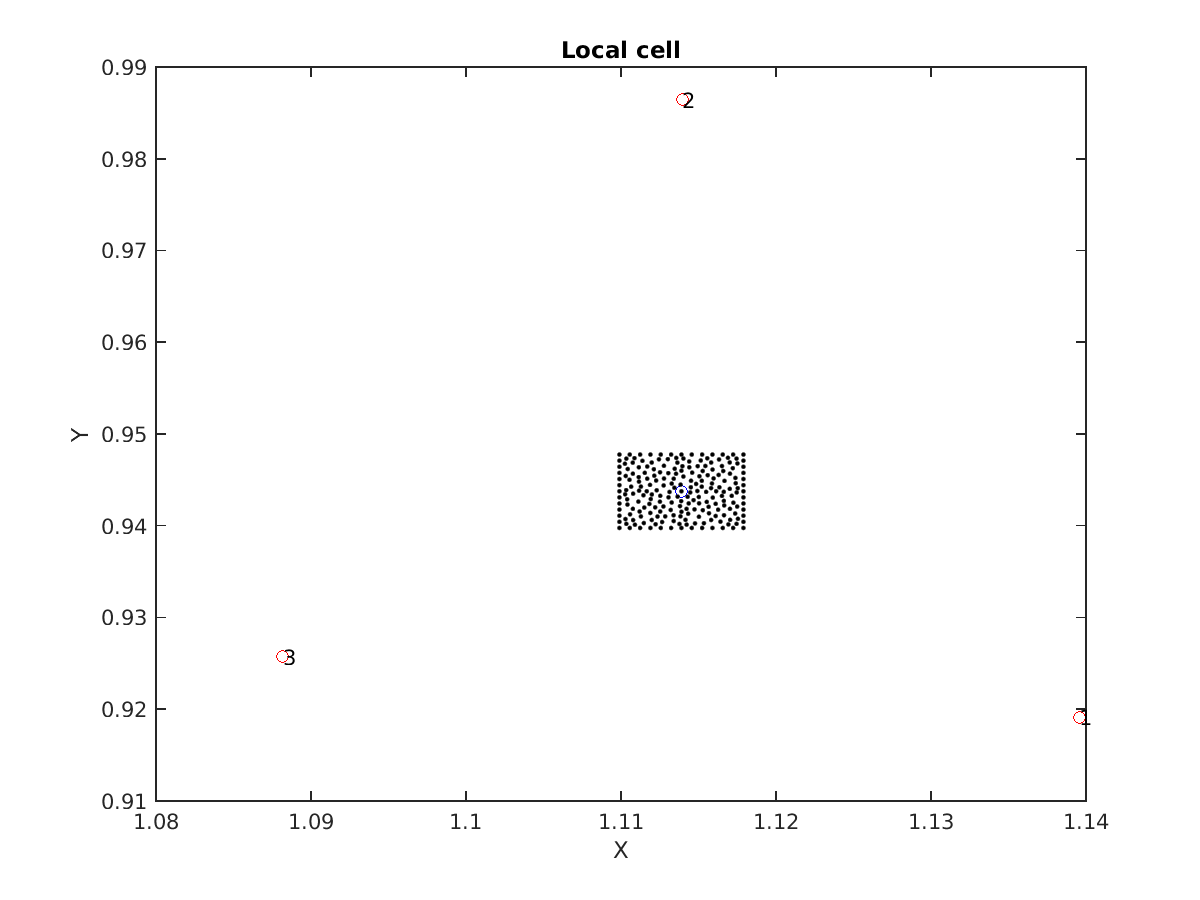
\includegraphics[width=.5\textwidth]{Code/local_cell.png} 
  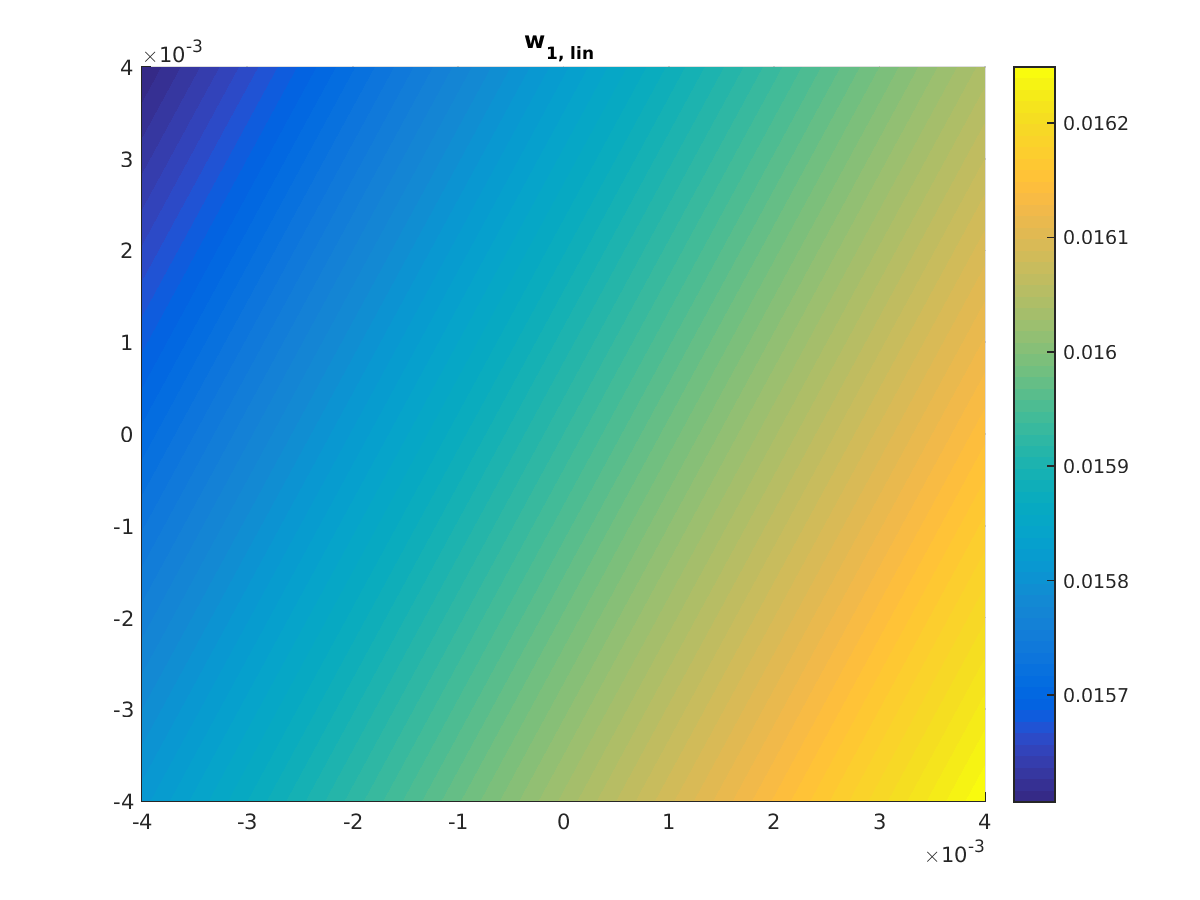
\includegraphics[width=.45\textwidth]{Code/w1lin.png} \\
  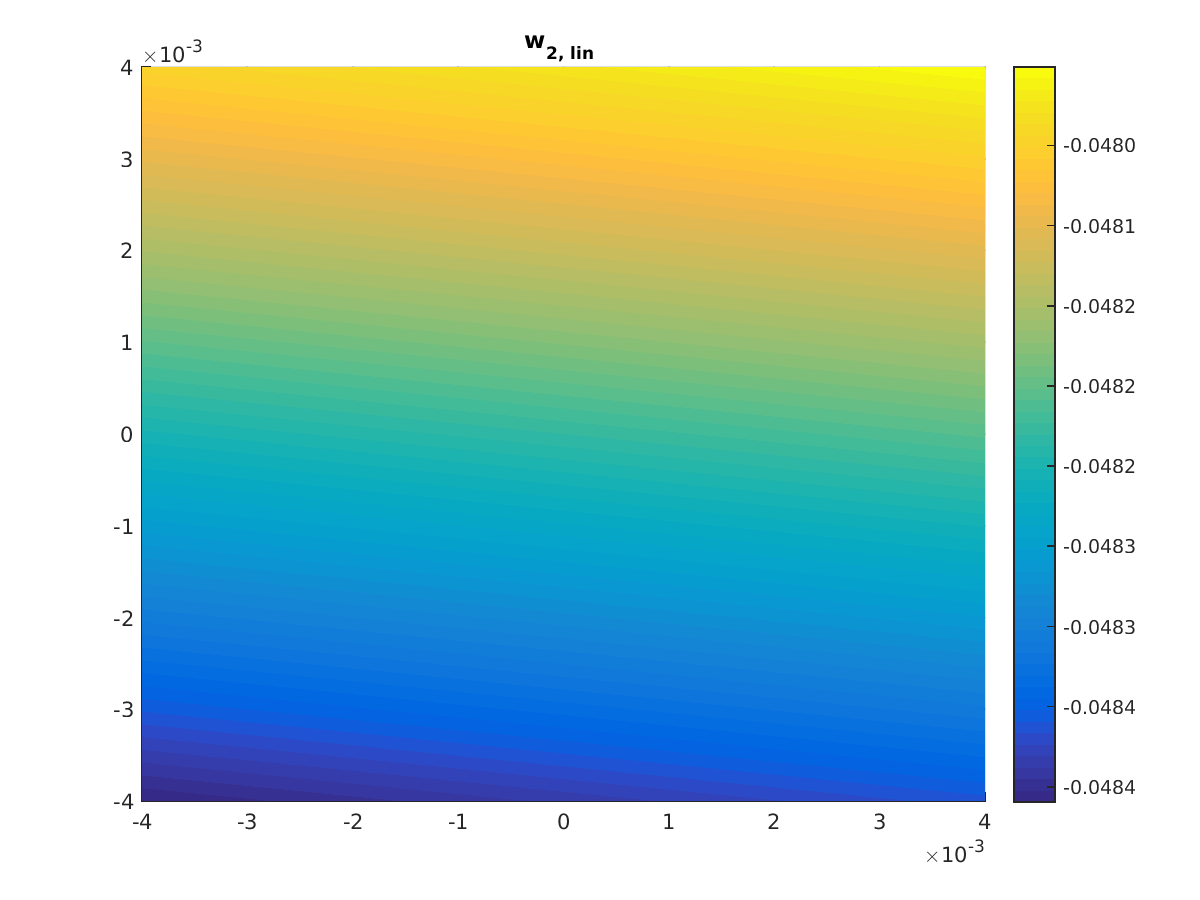
\includegraphics[width=.45\textwidth]{Code/w2lin.png}
  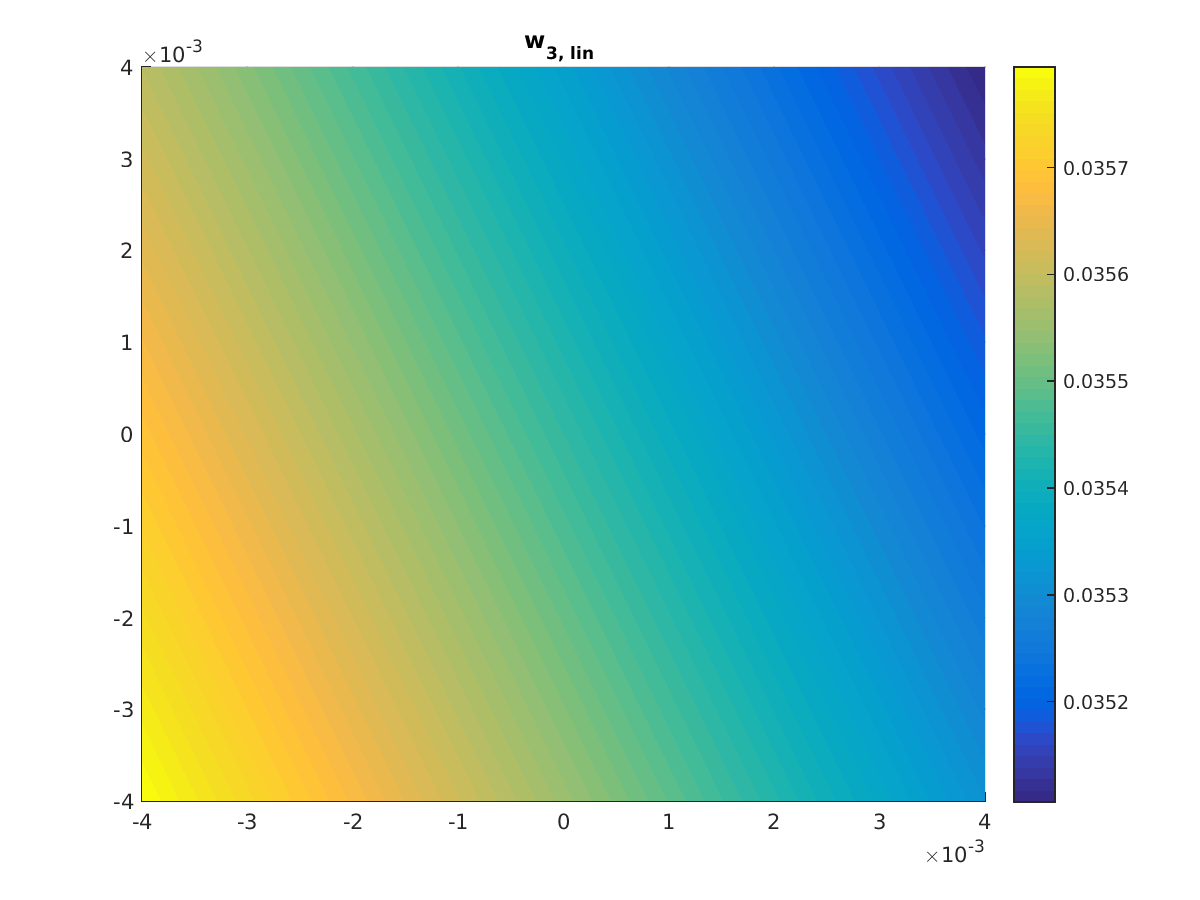
\includegraphics[width=.45\textwidth]{Code/w3lin.png}
  \caption{Projection des éléments de la macro-base sur les micro maillages. L'image de la cellule locale n'est pas très lisible, mais de gauche à
    droite on trouve les sommets 3, 2, 1 en rouge et le maillage est au centre. On voit en bleu le point de la quadrature. }
  \label{fig:wlins}
\end{figure}

\begin{figure}
  \centering
  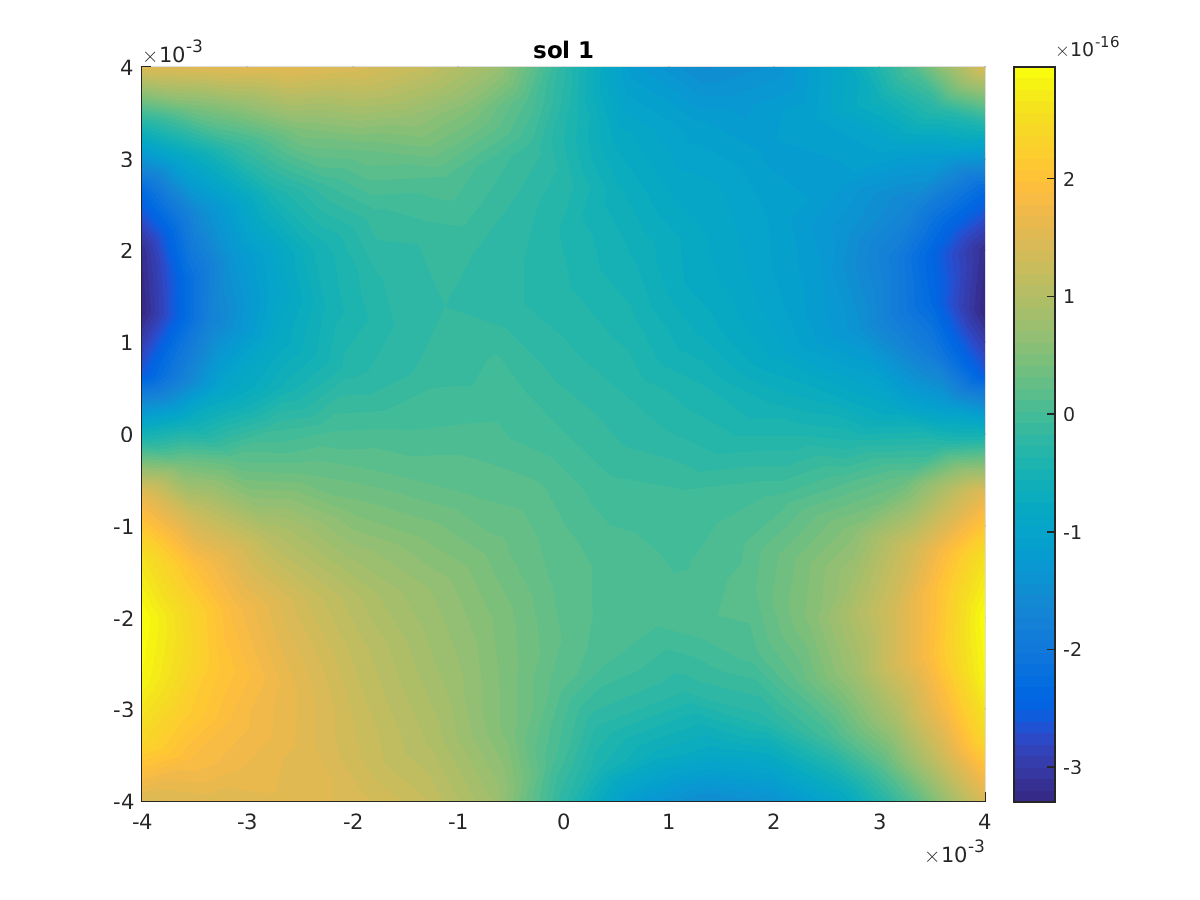
\includegraphics[width=.3\textwidth]{Code/w1.png} 
  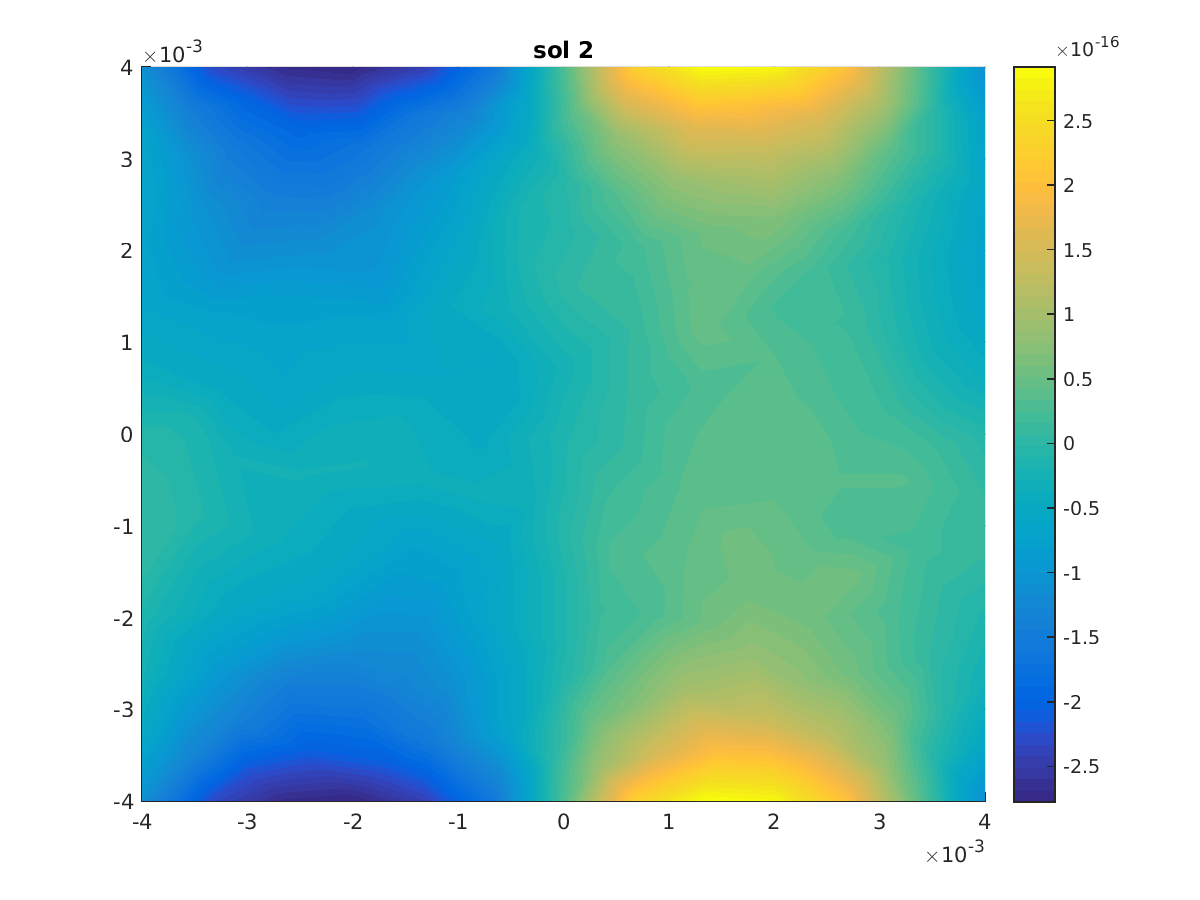
\includegraphics[width=.3\textwidth]{Code/w2.png}
  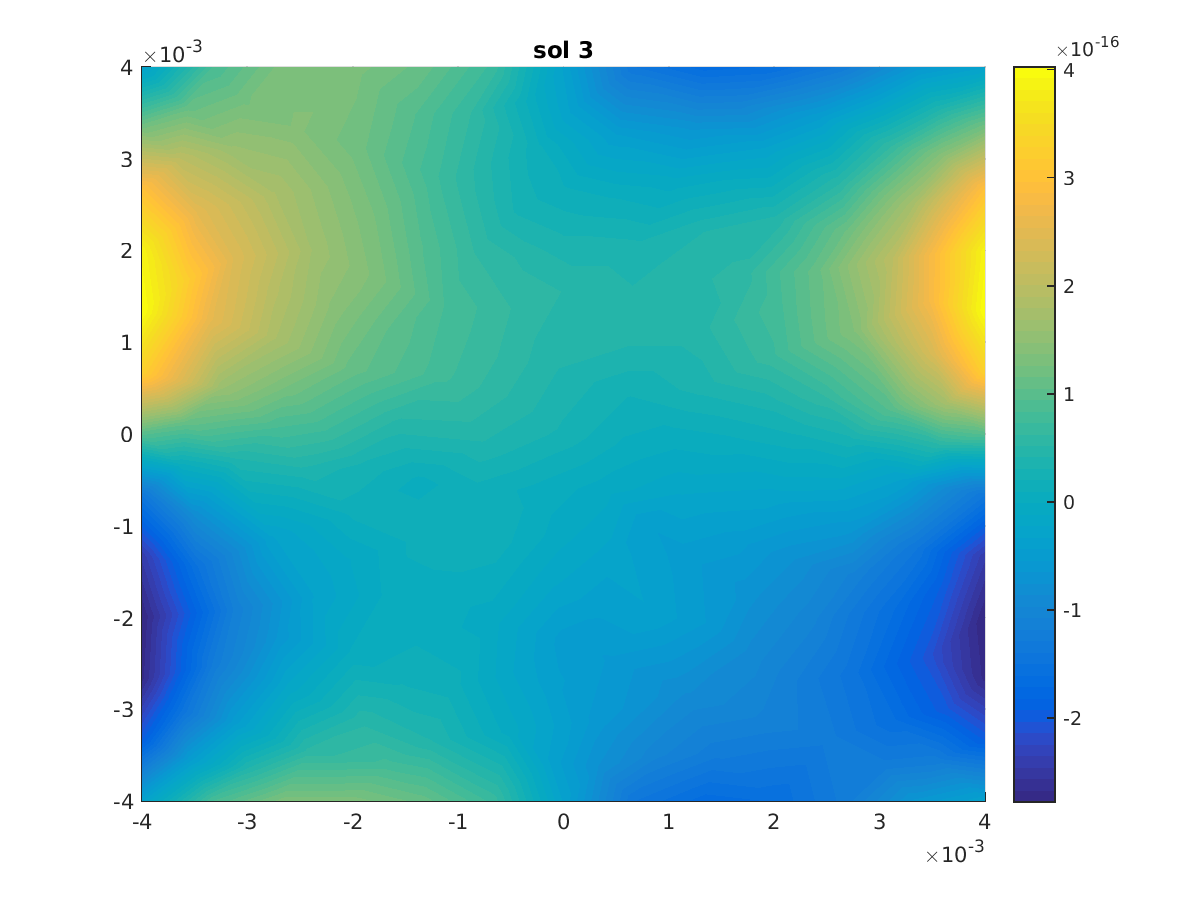
\includegraphics[width=.3\textwidth]{Code/w3.png} \\
  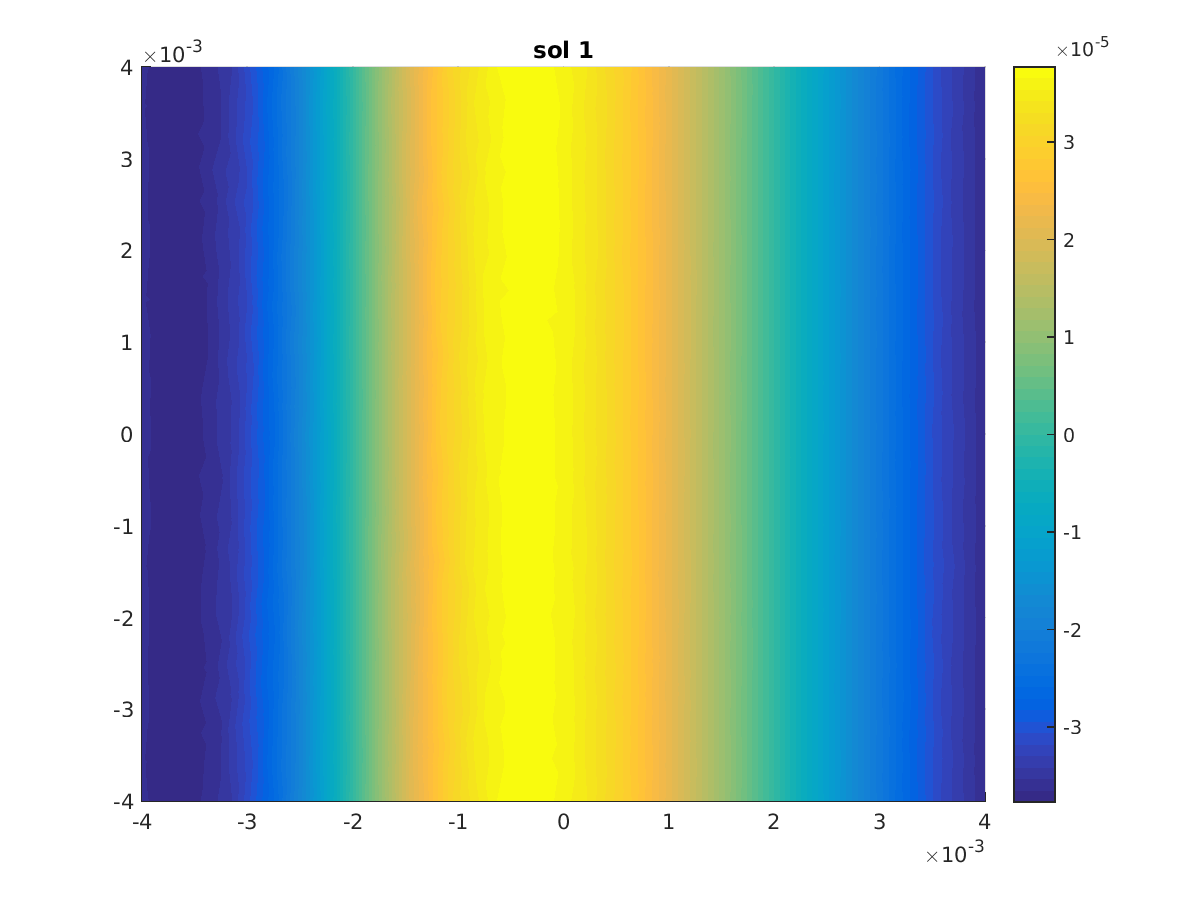
\includegraphics[width=.3\textwidth]{Code/w1_3.png} 
  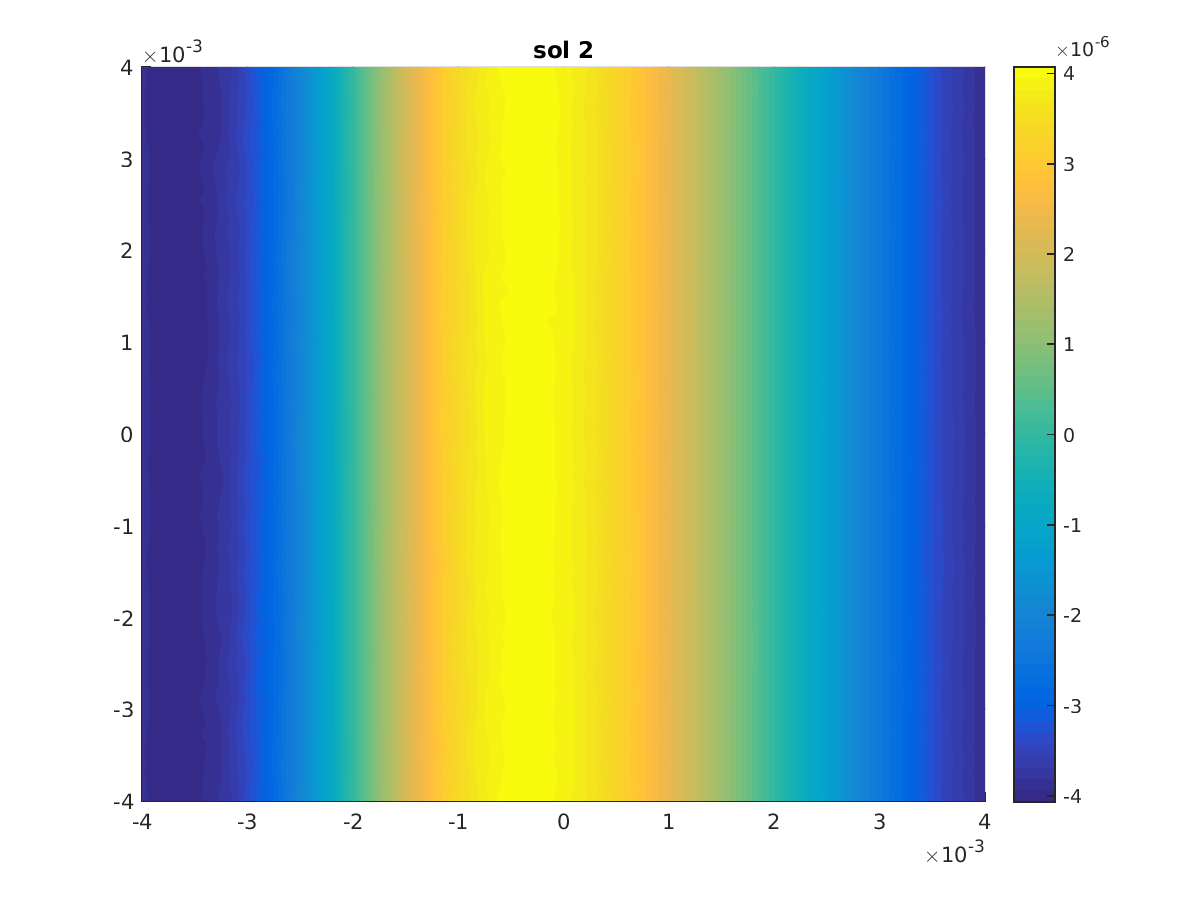
\includegraphics[width=.3\textwidth]{Code/w2_3.png}
  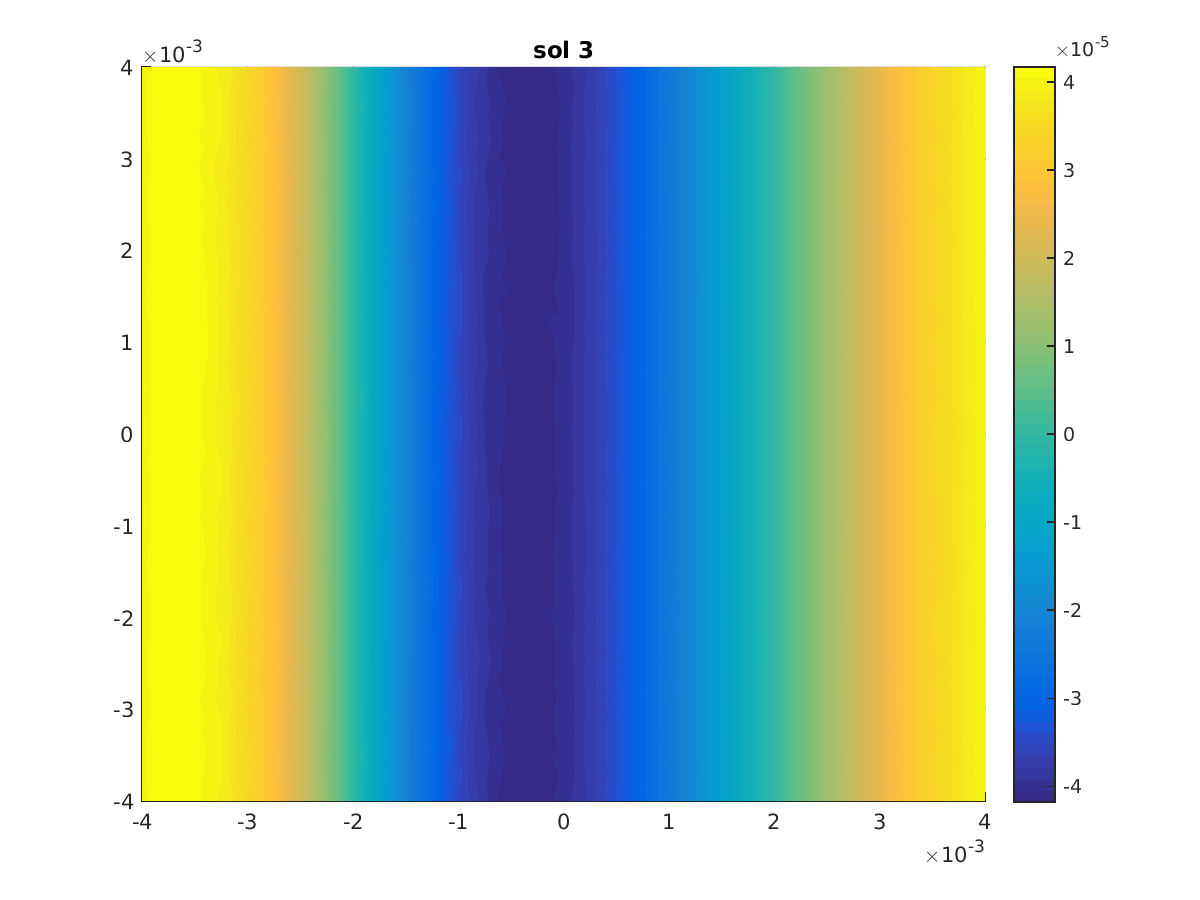
\includegraphics[width=.3\textwidth]{Code/w3_3.png} \\
  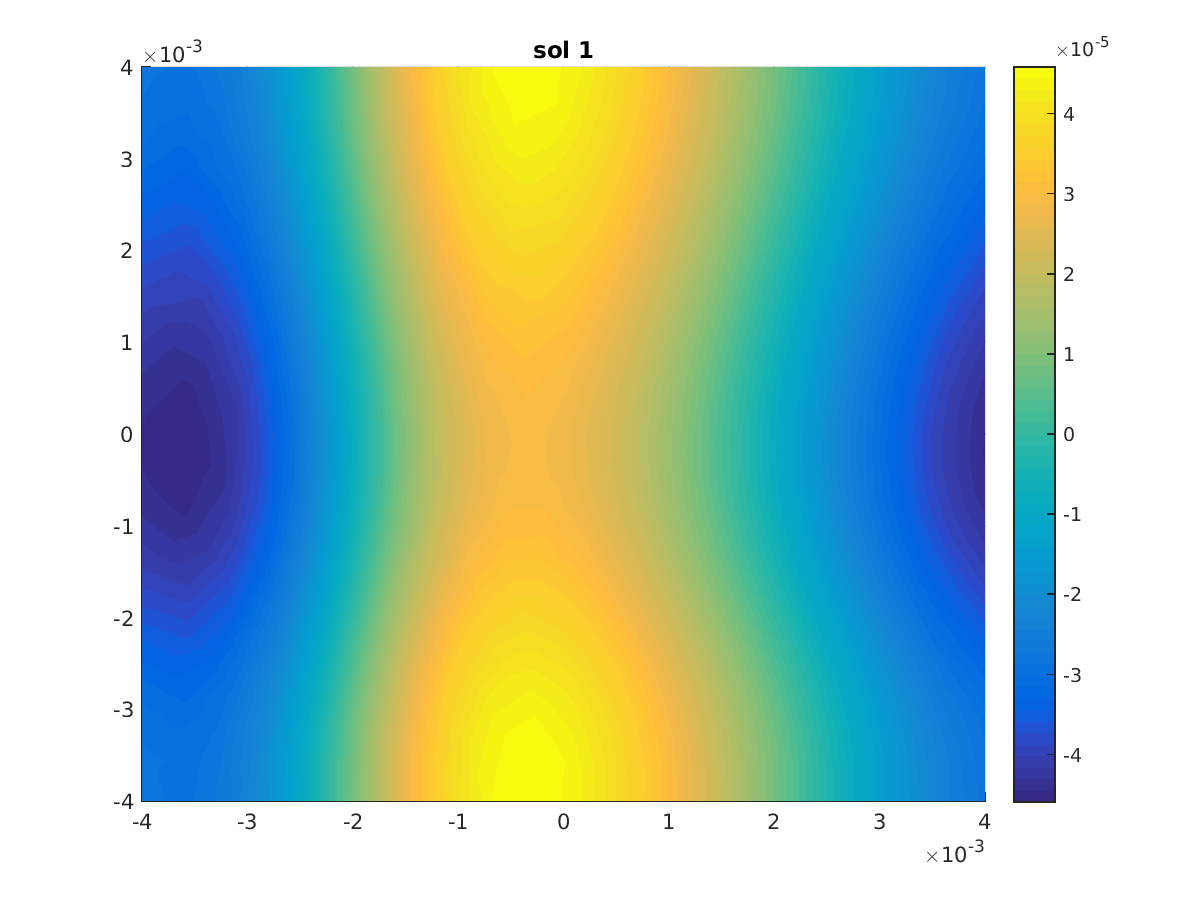
\includegraphics[width=.3\textwidth]{Code/w1_4.png} 
  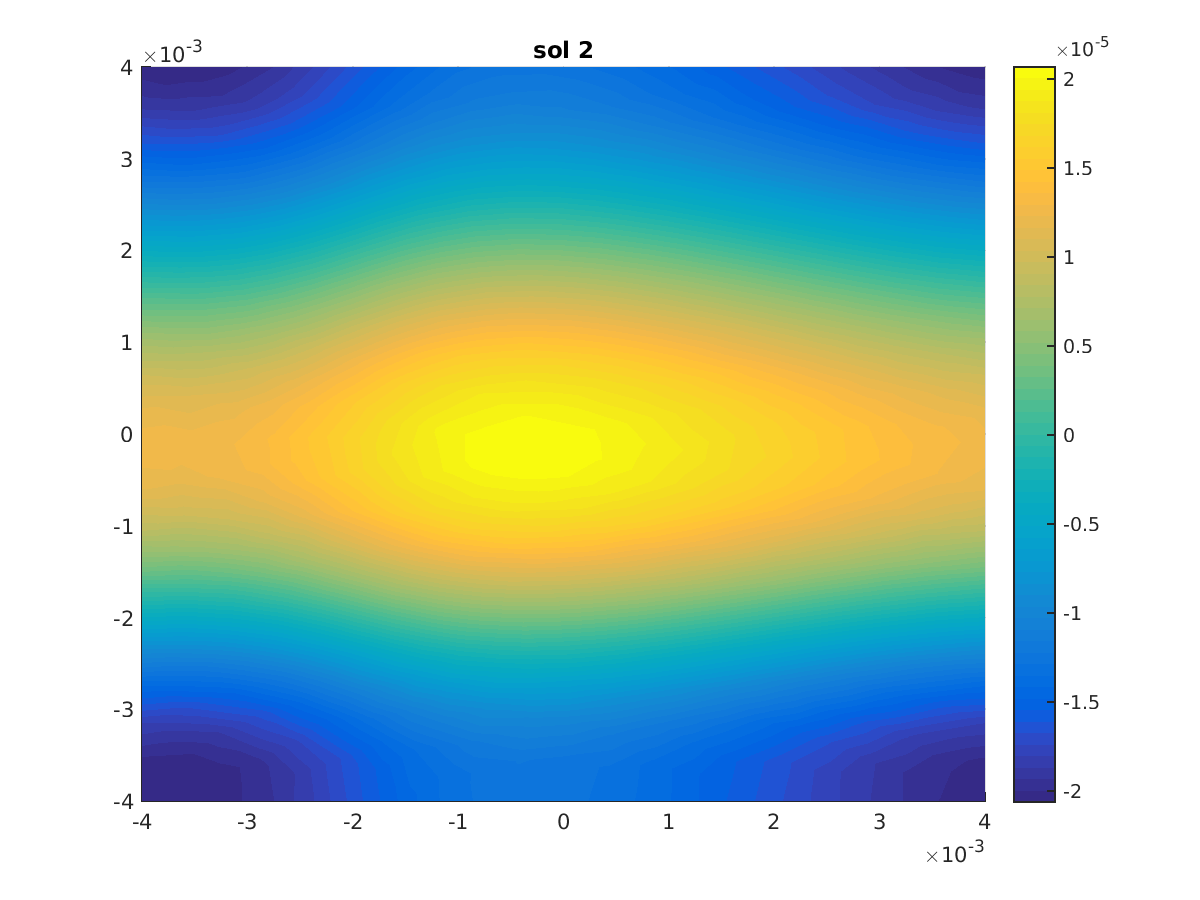
\includegraphics[width=.3\textwidth]{Code/w2_4.png}
  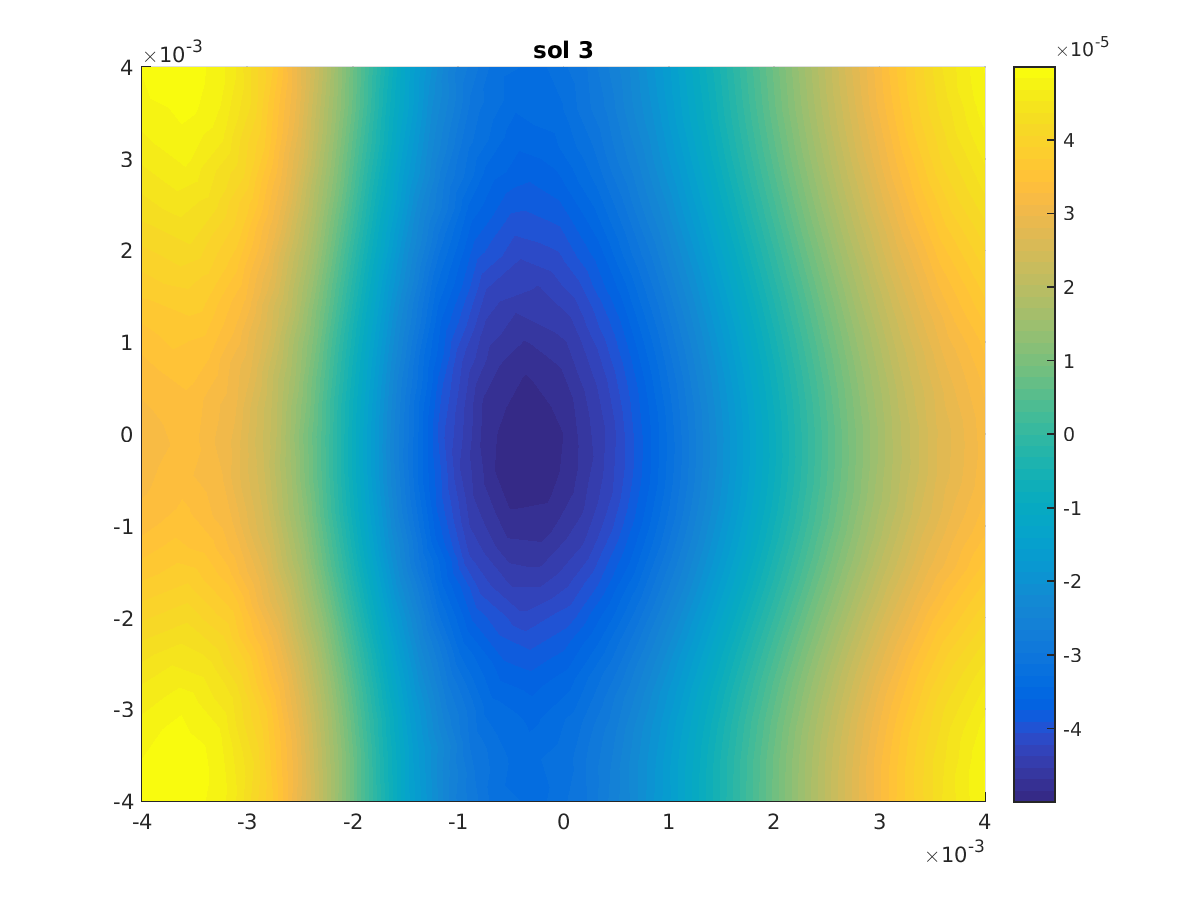
\includegraphics[width=.3\textwidth]{Code/w3_4.png} \\
  \caption{Solutions aux problèmes de cellule différencier avec leur élément de la macro-base locale. Première ligne, cas (i) du TP3, seconde ligne
    cas (iii) et troisième ligne cas(v). Le cas (ii) donne les mêmes résultats que (i) et le cas (iv) donne le même résultat que (iii). Encore une fois la lisibilité n'est pas au
    rendez-vous, mais l'ordre de grandeur est de $10^{-6}$ pour le cas (i) et $10^{-5}$ pour les autres cas.}
  \label{fig:ws}
\end{figure}

\begin{figure}
  \fbox{
  \begin{minipage}{\textwidth}
  \begin{itemize}
  \funcin \texttt{principal\_dirichlet\_aux}
  \item Lecture des maillages
  \funcin \texttt{calc\_constr\_mat}
  \item Constuction de la matrice de contraintes $\D$
  \funcout \texttt{calc\_constr\_mat}
  \loopin Pour macro-cellule dans le macro-maillage [PARALLELE]
  \setlength\itemindent{35pt}
  \funcin \texttt{calc\_constr\_mat}
  \item Calcul de la contribution de la cellule :
  \funcin \texttt{matK\_elem}
  \loopin Pour point dans quadrature
  \setlength\itemindent{70pt}
  \funcin \texttt{calc\_K\_contrib}
  \item Résoudre les trois problèmes modifiés
  \funcout \texttt{calc\_K\_contrib}
  \setlength\itemindent{35pt}
  \loopout Fin Pour point dans quadrature
  \item Sommer les valeurs de la quadrature
  \funcout \texttt{matK\_elem}
  \item Sauvegarder la contribution
  \item $\hdots$
  \setlength\itemindent{0pt}
  \loopout Fin Pour macro-cellule dans le macro-maillage
  \loopin Pour macro-cellule dans le macro-maillage [SEQUENTIELLE]
  \setlength\itemindent{35pt}
  \item Sommer les contributions des cellules pour construire les matrices de masse et rigidité
  \setlength\itemindent{0pt}
  \loopout Fin Pour macro-cellule dans le macro-maillage
  \item Résolution macro système
  \funcout \texttt{principal\_dirichlet\_aux}
  \end{itemize}
  \end{minipage}
  }
  \begin{itemize}
  \item [Légende]
  \item Opération classique
  \funcin Entrée dans une fonction
  \funcout Sortie d'une fonction
  \loopin Entrée dans une boucle
  \loopout [Fin $\hdots$] Sortie d'une boucle
  \end{itemize}
  \caption{Algorithme simplifié}
  \label{fig:algo}
\end{figure}


\begin{table}
  \centering
  \begin{tabular}{c|p{.5\textwidth}}
    Fonction                           & Usage                                                                                          \\
    \hline \hline
    \texttt{affiche}                   & Affiche une fonction sur un maillage                                                           \\
    \hline                 
    \texttt{affichemaillage}           & Affiche un maillage                                                                            \\
    \hline         
    \texttt{A}                         & Donne la valeur du tenseur $\Ae$ en $\xtk, \xtk/\varepsilon$                                   \\
    \hline                       
    \texttt{calc\_constr\_mat}         & Calcule la matrice de contrainte $\D$                                                          \\
    \hline         
    \texttt{calc\_K\_contrib}          & Calcule la contribution d'un point de la quadrature                                            \\
    \hline          
    \texttt{f}                         & Retourne le membre de droite pour le problème macro-scopique                                   \\
    \hline                 
    \texttt{lecture\_msh}              & Lecture d'un fichier \texttt{msh}                                                              \\
    \hline             
    \texttt{matK\_elem}                & Calcule la contribution d'une cellule à la matrice de rigidité globale                           \\
    \hline               
    \texttt{matK\_elem\_pbcell}        & Calcule la contribution d'une cellule à la matrice de rigidité micro                             \\
    \hline        
    \texttt{matM\_elem}                & Calcule la contribution d'une cellule à la matrice de masse globale                            \\
    \hline               
    \texttt{parfor\_progress}          & Utilitaire pour afficher l'avancement (trouvé sur le net)                                      \\
    \hline         
    \texttt{principal\_dirichlet\_aux} & Fonction principale de la résolution du problème macro et constructions de toutes les matrices \\
    \hline
    \texttt{principal\_dirichlet}      & Script principal d'appel                                                                       \\
    \hline     
  \end{tabular}
  \caption{Récapitulatif des fonctions du code}
  \label{tab:funcs}
\end{table}
\end{document}
%%% Local Variables:
%%% mode: latex
%%% TeX-master: t
%%% End:


% Après second changement de variable $x\rightarrow x +\bx$ on travaille avec les nouvelles fonctions $\eta_i = \varepsilon w_i(\bx, (x-\bx)/\varepsilon)$.
% On voudrait montrer que ces nouvelles fonctions résolvent le problème \autoref{eq:pbcelleta}

% pour cela, on peut résonner par équivalence en faisant le chemin inverse en faisant les changements de variables inverses
% \begin{enumerate}
% \item $x\rightarrow x+\bx$
% \item $x\rightarrow \varepsilon x$
% \end{enumerate}
% \begin{rmq}
%   Par des arguments de pseudo périodicité on peut montrer que le premier changement de variable ne change pas $A(x, x/\varepsilon)$.
% \end{rmq}

avec une disjonction de cas on trouve
\begin{equation}
  \begin{aligned}
    &\begin{cases}
      \int_{\Ye(\xtk)} A(\xtk, x/\varepsilon) B_1(\xtk, x/\varepsilon) (\nabla w_1)_1 \nabla_x \phi(x) dx = 0 \\
      \int_{\Ye(\xtk)} A(\xtk, x/\varepsilon) B_2(\xtk, x/\varepsilon) (\nabla w_1)_2 \nabla_x \phi(x) dx = 0 \\
    \end{cases} && l=1\\
    \text{et}~~
    &\begin{cases}
      \int_{\Ye(\xtk)} A(\xtk, x/\varepsilon)B_1(\xtk, x/\varepsilon) (\nabla w_2)_1 \nabla_x \phi(x) dx = 0 \\
      \int_{\Ye(\xtk)} A(\xtk, x/\varepsilon)B_2(\xtk, x/\varepsilon) (\nabla w_2)_2 \nabla_x \phi(x) dx = 0 \\ 
    \end{cases} && l=2\\
    \iff
    &\begin{cases}
      \int_{\Ye(\xtk)} A(\xtk, x/\varepsilon)B(\xtk, x/\varepsilon) \nabla w_1 \nabla_x \phi(x) dx = 0 \\
      \int_{\Ye(\xtk)} A(\xtk, x/\varepsilon)B(\xtk, x/\varepsilon) \nabla w_2 \nabla_x \phi(x) dx = 0 \\ 
    \end{cases} \\
    \iff
    &\begin{cases}
      \int_{\Ye(\xtk)} A(\xtk, x/\varepsilon)\nabla_x \tw_1(\xtk, x/\varepsilon) \nabla_x \phi(x) dx = 0 \\
      \int_{\Ye(\xtk)} A(\xtk, x/\varepsilon)\nabla_x \tw_2(\xtk, x/\varepsilon) \nabla_x \phi(x) dx = 0 \\ 
    \end{cases}
  \end{aligned}
\end{equation}